\documentclass[a4paper]{scrartcl}


\usepackage[utf8]{inputenc}
\usepackage[ngerman]{babel}
\usepackage{enumerate}
\usepackage{tikz}
\usepackage{fancyhdr}
\usepackage{lastpage}
\usepackage{verbatim}

\usepackage{listings}
\setlength{\parindent}{0mm}
\usepackage{graphicx}
\usepackage{amsmath}
\usepackage{algorithm2e}

\pagestyle{fancy}
\fancyhead[L]{Wintersemester\\2016/2017}
\fancyhead[C]{Enterprise Computing Praktikum\\Blatt 2}
\fancyhead[R]{Nikolas Zeitler\\Joshua Hartmann}

\fancyfoot[L]{}
\fancyfoot[C]{\thepage /\pageref{LastPage}}
\fancyfoot[R]{}

\renewcommand{\textheight}{700px}
\renewcommand{\footskip}{10px}
\newcommand*\xor{\mathbin{\oplus}}
\begin{document}
	\section{Aufgabe}
	\subsection{Screenshot von DSLIST}
	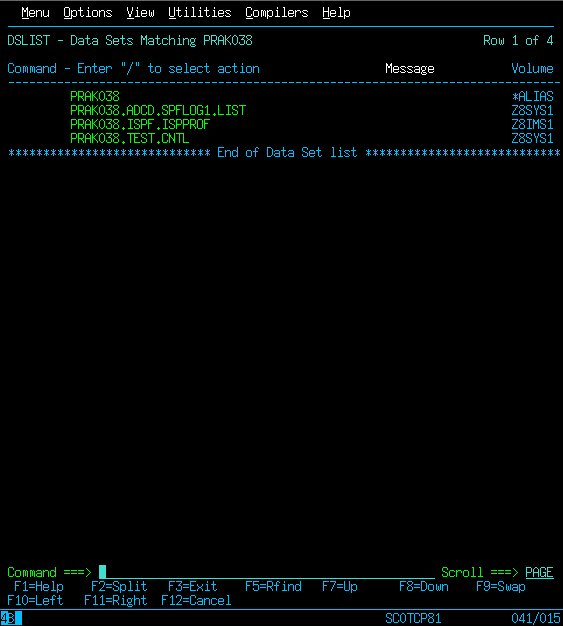
\includegraphics{screenshots/1_DSLIST.png}
	\section{Aufgabe}
	\subsection{Screenshot Sourcecode}
	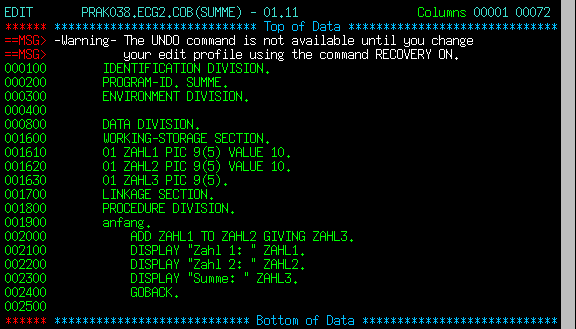
\includegraphics{screenshots/2_cobol_code.png}
	
	\subsection{Screenshot Programmausgabe}
	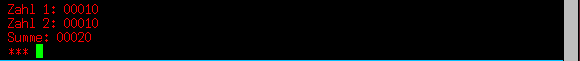
\includegraphics{screenshots/2_cobol_output.png}
	
	\subsection{Modifiziertes JCL Skript}
	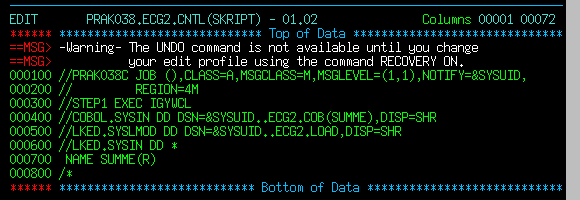
\includegraphics{screenshots/2_jcl_script.png}
	
	
	\subsection{Beschreibung des Programms:} 
	
	Unser Programm deklariert drei Variablen, die Zahlenwerte aufnehmen können. Zwei dieser Variablen wird ein Wert zugewiesen, die dritte dient als Platzhalter.\\
	Die Ausführung des Programms nimmt die ersten beiden Variablen, addiert die Werte und speichert das Ergebnis in der dritten Variable. Anschließend gibt das Programm die Summanden sowie die Summe aus.
	
	
	
	\section{Aufgabe}
	\subsection{Screenshot von Fehler}
	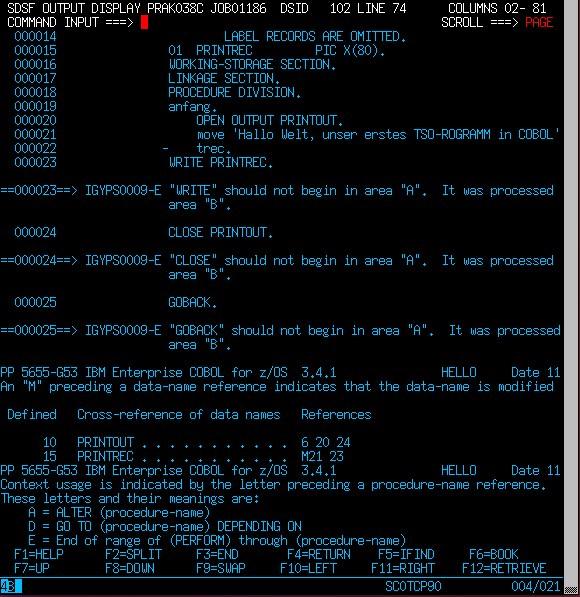
\includegraphics{screenshots/3_sdsf_error.png}
	
	\subsection{Was würde passieren, wenn sie Ihren laufenden TSUXXXXX-Job purgen würden?}
	
	Wahrscheinlich würde das unsere Session auf dem System beenden und wir würden damit die Verbindung verlieren.
\end{document}

